% ============================================================================
%  Section: DID Recovery Scaling Across Institutions
%
%  Measures the cost of the user-facing DID-recovery flow as a function of
%  the number of salt-custodian institutions N (3, 5, 7, 9, 11). Recovery
%  excludes the prover and on-chain submission paths — it only requires
%  re-authenticating with the OAuth provider and re-fetching salt shares
%  to deterministically reconstruct the patient's zkLogin DID.
%
%  Required packages:
%    \usepackage{graphicx}
%    \usepackage{booktabs}
%
%  Required figure files:
%    figures/fig_recovery_scaling.pdf
% ============================================================================

\subsubsection{DID Recovery Scaling}
\label{sec:did-recovery}

Sections~\ref{sec:e2e-timing}--\ref{sec:ehr-access} characterize the
\emph{enrollment} path — registering a new DID and issuing access
grants. A complementary scenario is \emph{recovery}: a patient who has
lost their wallet device must re-obtain their DID by re-authenticating
with their OAuth provider and re-fetching salt shares from the
custodian institutions. Because the zkLogin address is a deterministic
function of \texttt{(iss, aud, sub, salt)} and the salt is itself
deterministic per \texttt{(institution\_seed, sub)}, recovery does
\emph{not} require any blockchain interaction or ZK proof: it consists
solely of an OAuth round-trip, an N-way parallel salt fan-out, and one
local \texttt{jwtToAddress} hash. We measure how this recovery latency
scales with the number of salt-custodian institutions.

% ----------------------------------------------------------------------------
% Methodology
% ----------------------------------------------------------------------------
\paragraph{Methodology}

We deployed eleven independent salt-services across two AWS regions: one
co-located with the browser host on \texttt{us-east-1} (loopback path,
serving as ``Institution~1''), and ten on individual public EC2 instances
in \texttt{us-west-1} (Institutions~2--11), accessed via real cross-region
public-network paths. The auth.ts library exposes a \texttt{?mode=recovery}
URL parameter that instructs the post-OAuth pipeline to skip the ZK
prover request and the bridge session upload — the flow stops once the
zkLogin DID has been computed locally from JWT plus merged salt. The
Playwright observer measures \texttt{wall\_login} as the wall-clock
interval from the user's \emph{Login with Google} click to the
\emph{``Logged in as ...''} toast, which under recovery mode brackets
exactly \{OAuth round-trip\}\,$+$\,\{N-way salt fan-out\}\,$+$\,\{local DID
derivation\}\,$+$\,\{browser-side bookkeeping\}.

For each $N \in \{3, 5, 7, 9, 11\}$ we ran $n=30$ recovery trials with
fresh per-trial state (the page is closed and reopened, sessionStorage and
localStorage are wiped, only the Google OAuth cookie persists; a fresh
JWT is therefore issued by Google every trial). The selected
institution set always includes Institution~1 (loopback) plus
$N{-}1$ cross-region institutions, matching a realistic deployment
where one custodian is geographically close and the rest are remote.
All 150 trials succeeded. The persistent backend worker
(\S\ref{sec:session-reuse}) is not exercised in this experiment because
the recovery flow has no Node-side path — Vite serves the static client
and the eleven salt-services answer JSON requests directly.

% ----------------------------------------------------------------------------
% Results
% ----------------------------------------------------------------------------
\paragraph{Results}

Table~\ref{tab:recovery-scaling} reports per-$N$ statistics, and
Figure~\ref{fig:fig_recovery_scaling} visualizes the salt-fetch
distribution and total \texttt{wall\_login} as $N$ grows.

\begin{table}[h]
\centering
\small
\caption{DID recovery wall-clock and per-phase latency as a function of
the number of salt-custodian institutions $N$ ($n=30$ each, all in ms).
\emph{Salt fetch} denotes the parallel \texttt{Promise.all} fan-out;
\emph{prover} and \emph{bridge\_post} are confirmed zero by construction.}
\label{tab:recovery-scaling}
\begin{tabular}{rrrrrrrr}
\toprule
\textbf{N} & \textbf{phase}     & \textbf{mean} & \textbf{sd} & \textbf{p50} & \textbf{p95} & \textbf{min} & \textbf{max} \\
\midrule
3  & \texttt{wall\_login} & 1{,}092 & 204 &    968 & 1{,}395 &    925 & 1{,}582 \\
3  & oauth\_rtt           &    662 &  43 &    658 &    700 &    598 &    860 \\
3  & salt fetch           &     90 &  34 &     66 &    127 &     65 &    189 \\
\addlinespace
5  & \texttt{wall\_login} & 1{,}099 & 253 &    952 & 1{,}374 &    904 & 1{,}983 \\
5  & oauth\_rtt           &    660 &  29 &    655 &    689 &    628 &    793 \\
5  & salt fetch           &    126 & 111 &    124 &    129 &     64 &    697 \\
\addlinespace
7  & \texttt{wall\_login} & 1{,}088 & 244 &    957 & 1{,}390 &    918 & 1{,}945 \\
7  & oauth\_rtt           &    654 &  13 &    653 &    676 &    633 &    688 \\
7  & salt fetch           &    124 & 145 &    128 &    130 &     66 &    877 \\
\addlinespace
9  & \texttt{wall\_login} & 1{,}107 & 232 &    971 & 1{,}380 &    906 & 1{,}784 \\
9  & oauth\_rtt           &    654 &  16 &    655 &    677 &    615 &    691 \\
9  & salt fetch           &    136 & 140 &    129 &    131 &     68 &    867 \\
\addlinespace
11 & \texttt{wall\_login} & 1{,}083 & 246 &    956 & 1{,}360 &    892 & 1{,}955 \\
11 & oauth\_rtt           &    653 &  18 &    658 &    674 &    620 &    703 \\
11 & salt fetch           &    137 & 138 &    131 &    133 &     68 &    857 \\
\bottomrule
\end{tabular}
\end{table}

\begin{figure}[h]
\centering
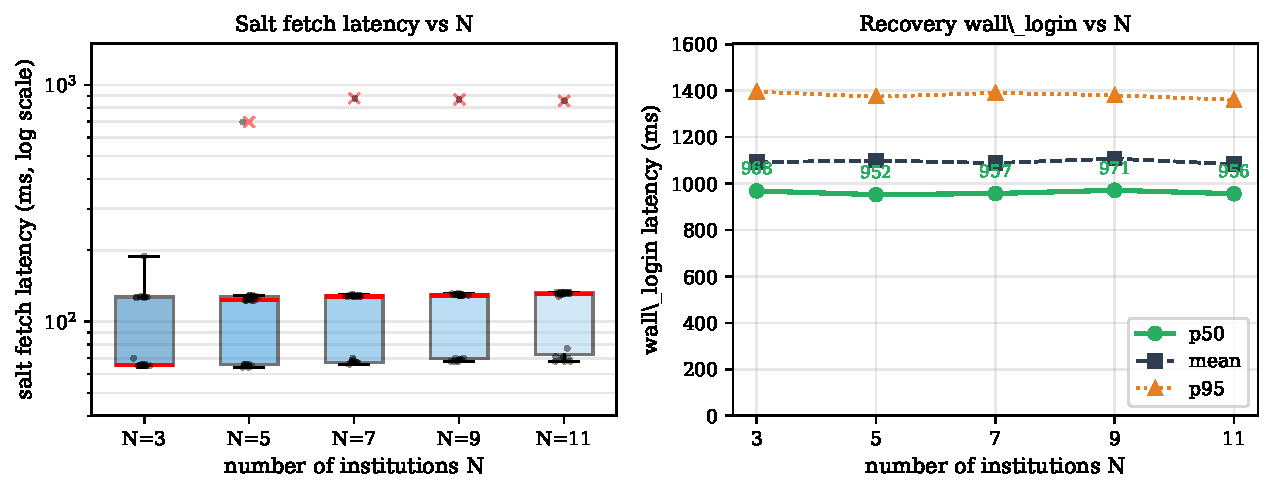
\includegraphics[width=\linewidth]{figures/fig_recovery_scaling.pdf}
\caption{DID recovery scaling with the number of institutions $N$ ($n=30$
trials per $N$). \textbf{Left}: salt-fetch latency distribution
(boxplot, log scale). The medians plateau at 124--131\,ms for $N \ge 5$
because parallel \texttt{Promise.all} fan-out is bounded by the slowest
of $N$ concurrent requests, which is one cross-region RTT regardless
of $N$. The cold-start outliers (700--880\,ms) reflect first-fetch
TLS handshakes to recently-deployed institutions and are independent
of $N$. \textbf{Right}: \texttt{wall\_login} median, mean, and p95
versus $N$. The total recovery latency is essentially flat across
$N \in [3, 11]$, with median 952--971\,ms.}
\label{fig:fig_recovery_scaling}
\end{figure}

% ----------------------------------------------------------------------------
% Discussion
% ----------------------------------------------------------------------------
\paragraph{Discussion}

The experiment yields three findings of practical relevance to threshold
salt-custodian deployments.

\textbf{(i)~Recovery latency is essentially $N$-invariant.} Median
\texttt{wall\_login} is 952--971\,ms across all five values of $N$
(range: 19\,ms, well within trial-to-trial variance). Adding eight
additional salt-custodian institutions to the recovery path (from $N=3$
to $N=11$) imposes no measurable user-facing latency cost. This is the
expected behavior under \texttt{Promise.all} fan-out — total wall time
is $\max_i \text{RTT}_i$, not $\sum_i \text{RTT}_i$ — but our measurement
confirms that browser-level connection-pool effects and TLS
parallelism do not break this property at $N=11$.

\textbf{(ii)~Salt fetch median is bounded by single-host cross-region
RTT.} The salt-phase medians cluster at 124--131\,ms for $N \in
\{5, 7, 9, 11\}$, matching the
\texttt{us-east-1}\,$\leftrightarrow$\,\texttt{us-west-1} steady-state
RTT measured in \S\ref{sec:module-salt}. The $N=3$ case is faster
(p50 = 66\,ms) because it includes only two cross-region hops and one
loopback; for $N \ge 5$ at least four parallel cross-region requests
are issued and the median reliably tracks the single-host
cross-region RTT.

\textbf{(iii)~OAuth round-trip dominates recovery latency.} OAuth
contributes $\sim$655\,ms (60\,\% of \texttt{wall\_login} median);
salt contributes 124--131\,ms (13\,\%); the remaining $\sim$170\,ms is
browser-platform overhead (page mount, OAuth fragment parse, React
re-render, toast detection). Reducing recovery latency below 1\,s
therefore requires reducing the OAuth round-trip itself — for example
by switching to a popup-mode OAuth client, or to a provider with
lower latency than Google's account servers — rather than reducing the
number of salt custodians.

% ----------------------------------------------------------------------------
% Threshold-recovery implications
% ----------------------------------------------------------------------------
\paragraph{Implication for Threshold Custodianship}

A salt-derivation scheme that uses $t$-of-$N$ threshold reconstruction
(rather than the all-required SHA-256 merge measured here) gains a
robustness benefit at no measurable latency cost up to $N=11$: under
\texttt{Promise.all} fan-out the user pays the latency of the
$t$-th-fastest custodian rather than the slowest, which is bounded above
by the slowest custodian's RTT measured here ($\sim$130\,ms p50). For
deployments where individual custodian availability is the operative
constraint, scaling $N$ to 11 (or higher, by extrapolation from this
flat curve) is essentially free in user-facing latency.
